\begin{table*}[!t]
  \caption{Datasets description for infinite boosting and gradient boosting comparison}
  \label{tab:gb-data}
  \centering
  \dospace
  \begin{tabular}{lllll}
    \toprule
    Type     &  Name & Number of instances     & Number of features & Source \\
    \midrule
    classification & Higgs 1M & 1,500,000  & 28   & \href{https://archive.ics.uci.edu/ml/datasets/HIGGS}{\underline{link}}  \\
    regression     & YearPredictionMSD & 515,345 & 90   & \href{https://archive.ics.uci.edu/ml/datasets/YearPredictionMSD}{\underline{link}}   \\
    ranking     & yahoo-letor, set 1 &  638,794   & 699  & \cite{key-yahoo-data} \\
    \bottomrule
  \end{tabular}
\end{table*}

\begin{figure*}[!h]
  \centering
  \begin{multicols}{2}
    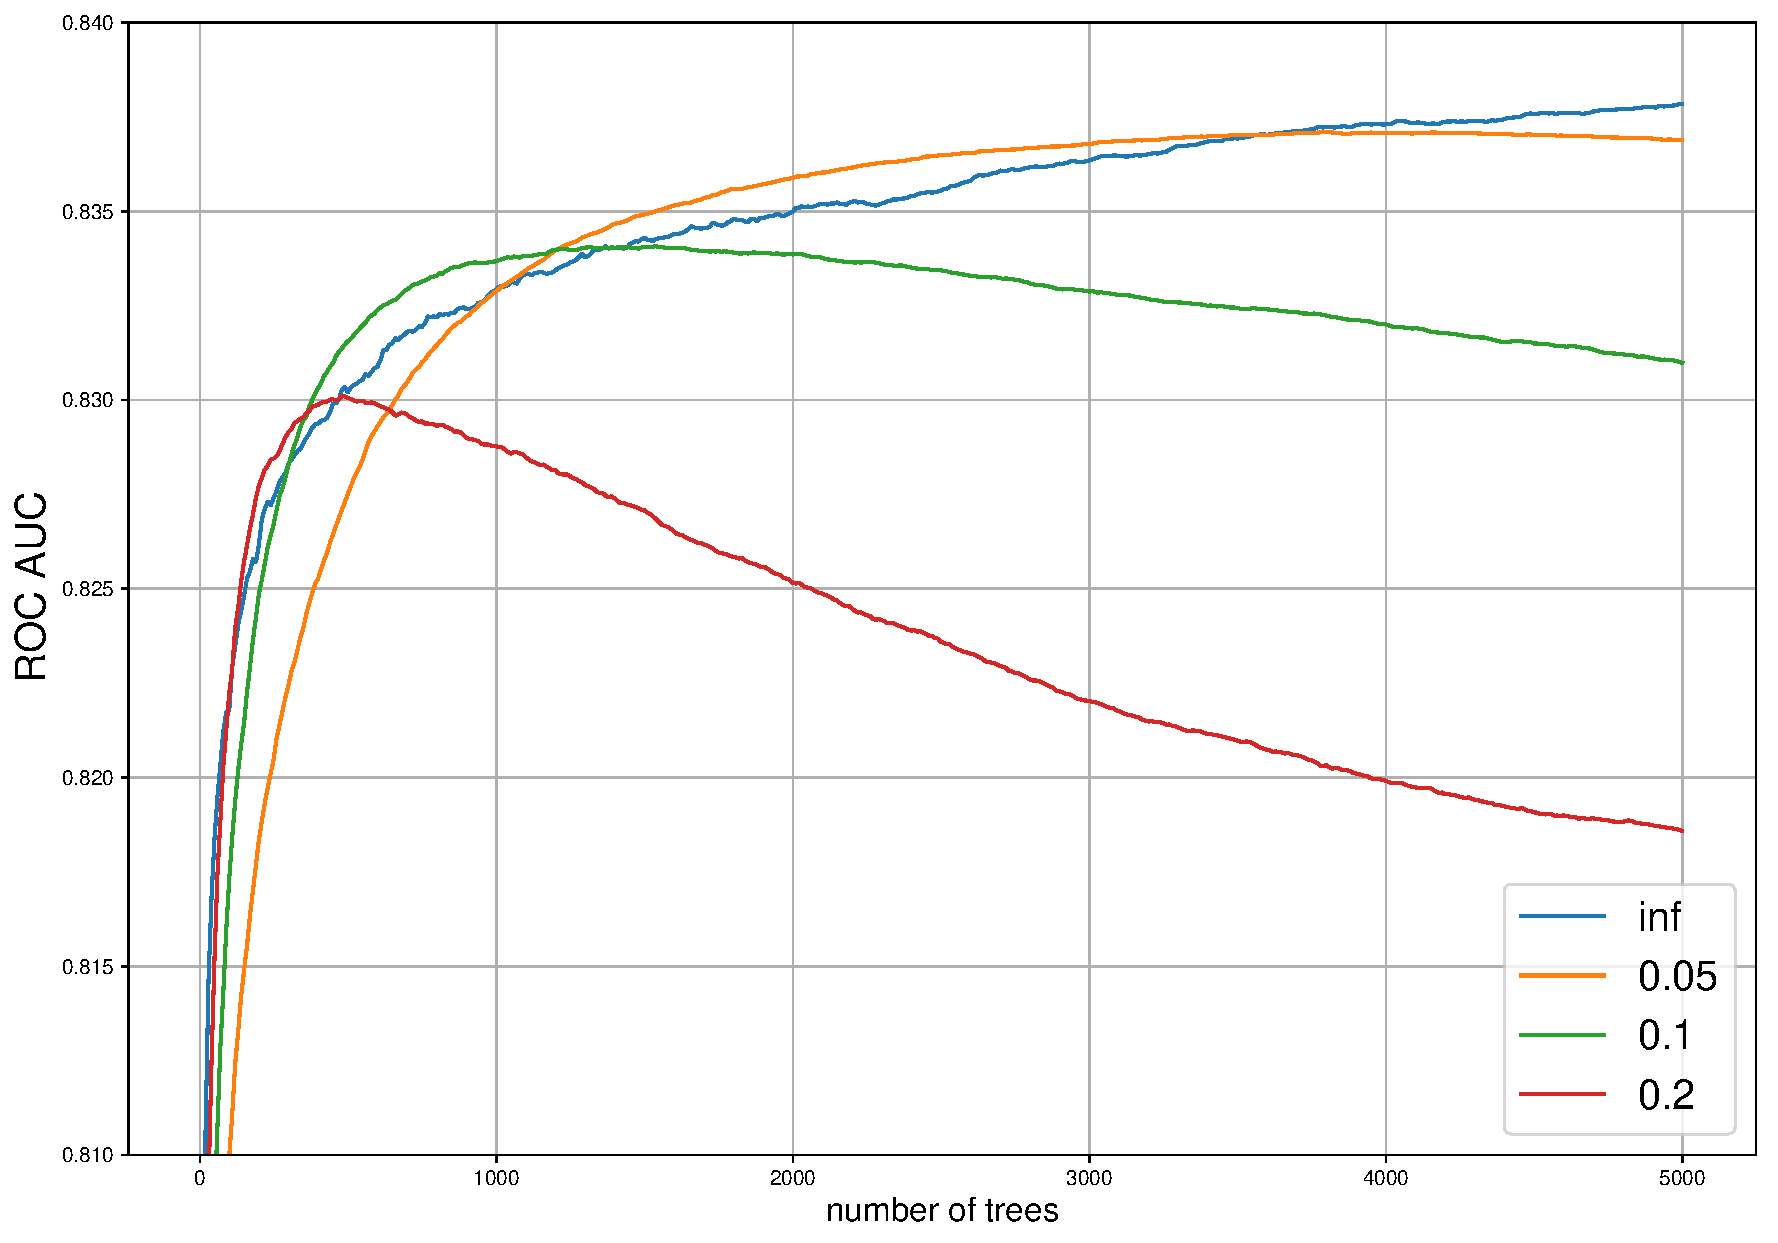
\includegraphics[width=1\linewidth]{../research/plots/rocauc_higgs.pdf}
    \caption{Quality on Higgs dataset for gradient boosting with different shrinkages ($0.05, \, 0.1,\, 0.2$) and infinite boosting with adaptive capacity (inf). \label{fig:gb-auc}}
    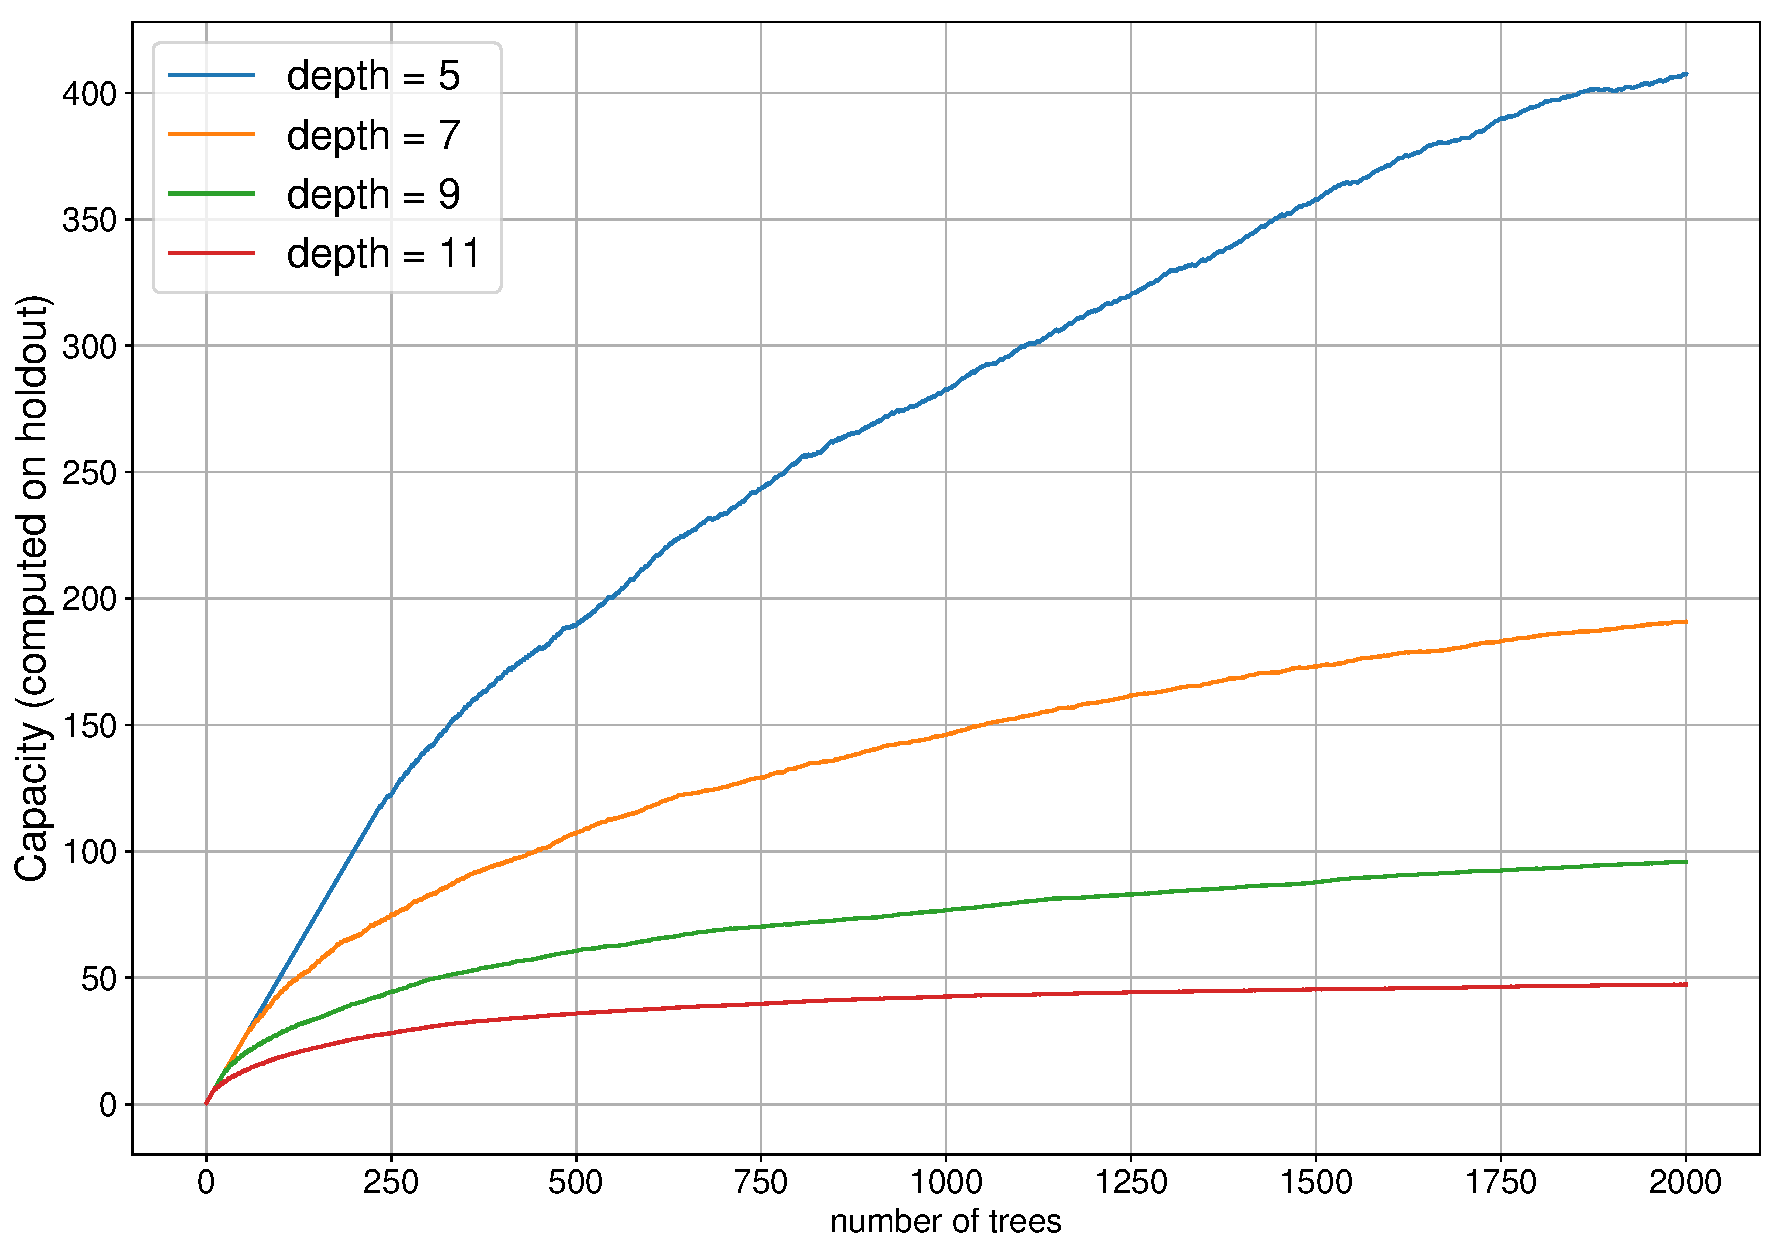
\includegraphics[width=1\linewidth]{../research/plots/various_depths_higgs.pdf}
    \caption{Comparison of infinite boost capacities found by adapting capacity on a holdout for different depths on Higgs dataset. \label{fig:gb-depth}}
  \end{multicols}
\end{figure*}

\begin{figure*}[!h]
  \centering
  \begin{multicols}{2}
    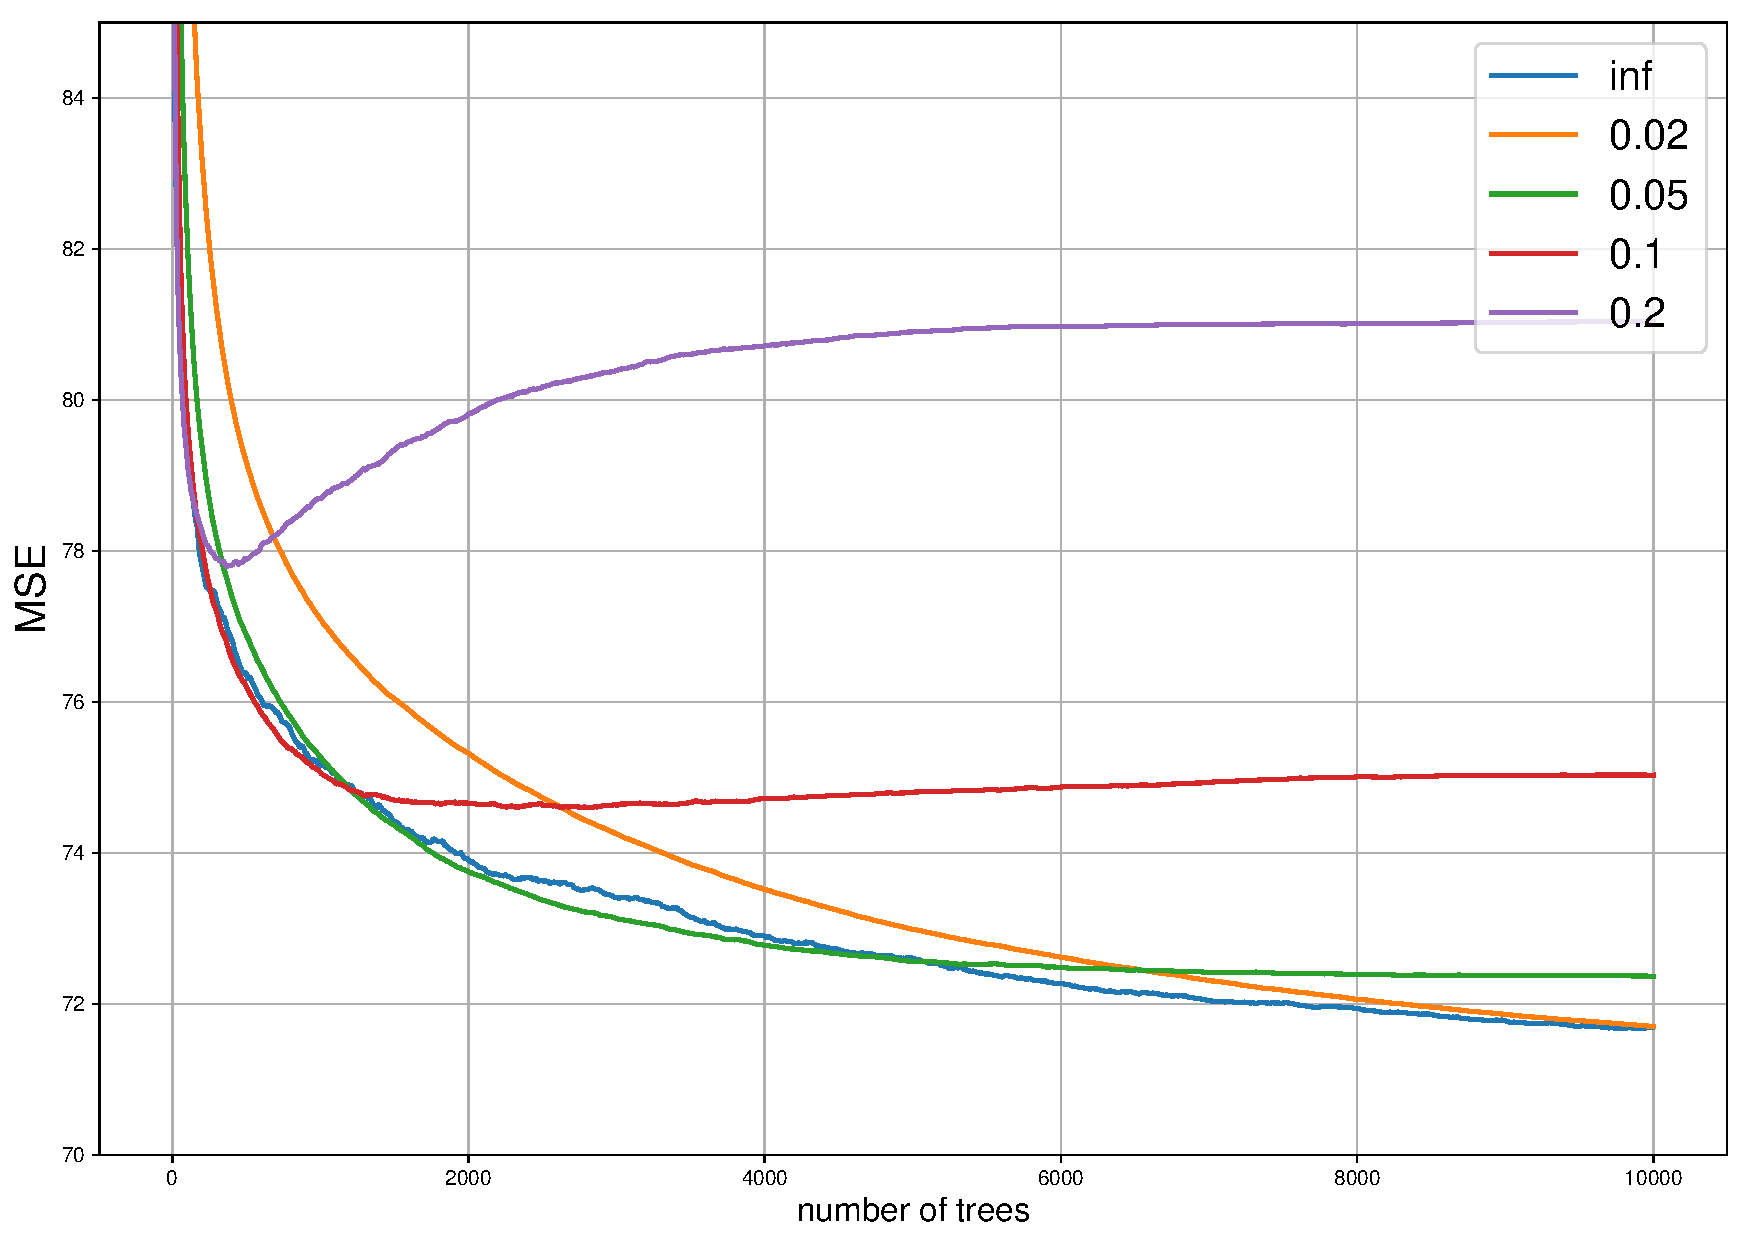
\includegraphics[width=1\linewidth]{../research/plots/songs_mse.pdf}
    \caption{Quality on YearPredictionMSD dataset for gradient boosting with different shrinkages ($0.02,\, 0.05, \, 0.1,\, 0.2$) and infinite boosting with adaptive capacity (inf). \label{fig:gb-mse}}
    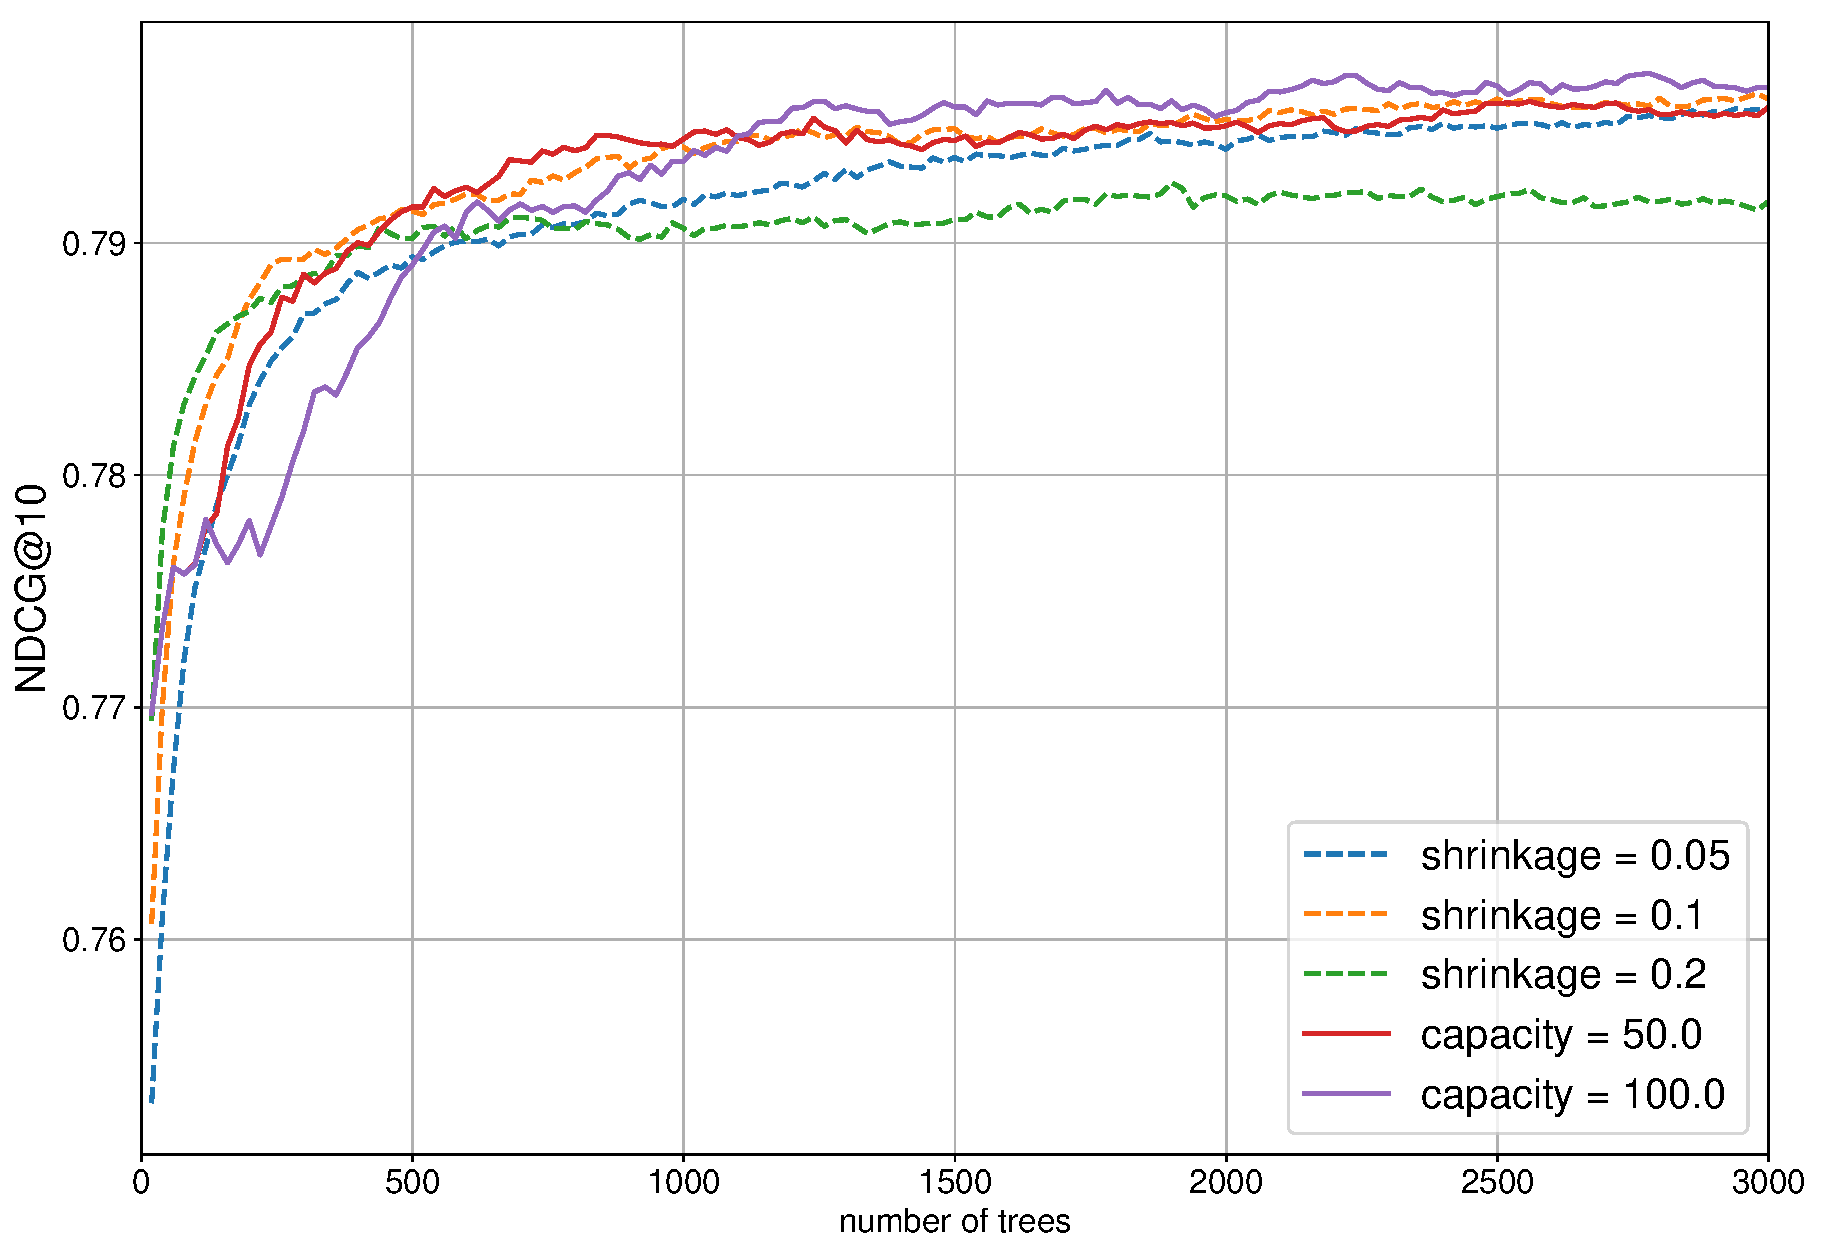
\includegraphics[width=1\linewidth]{../research/plots/ndcg_at_10.pdf}
    \caption{Quality on yahoo-letor dataset for gradient boosting with different shrinkages ($0.05, \, 0.1,\, 0.2$) and infinite boosting with different capacity values ($50,\, 100,\, 200$).
             Other NDCG@k plots can be found in supplementary material. \label{fig:gb-ndcg}}
  \end{multicols}
\end{figure*}
